\chapter{Een semantiek voor UML-klassediagrammen en controle op consistentie en kwaliteitsgebreken}\label{sec:consistentie}
Sectie \ref{sec:cd-components} geeft een beschrijving van de verscheidene componenten in een klassediagram die we beschouwen in deze masterproef. Die beschrijving gebruiken we om een modelsemantiek te defini\"eren voor klassediagrammen in sectie \ref{sec:cd-semantics}. Op basis van deze semantiek defini\"eren we consistentie en inconsistentie van een klassediagram. Sectie \ref{sec:cd-rep-cons} beschrijft een methode om een voorstellingswijze voor klassediagrammen in FO($\cdot$) te bekomen die overeenkomt met die semantiek. Zo kunnen we in sectie \ref{sec:cons-verify} consistentie en bepaalde soorten inconsistentie van een klassediagram nagaan. Tenslotte beschrijft sectie \ref{sec:kwaliteitsgebrek} een alternatieve voorstellingsmethode voor klassediagrammen om bepaalde soorten kwaliteitsgebrekken op te sporen.

\section{Componenten van een klassediagram}\label{sec:cd-components}

We gebruiken figuren \ref{fig:voorbeeld1} en \ref{fig:voorbeeld2} ter illustratie van de componenten in een klassediagram, die we beschrijven in de volgende subsecties.

\begin{figure}[h]
	\centering
	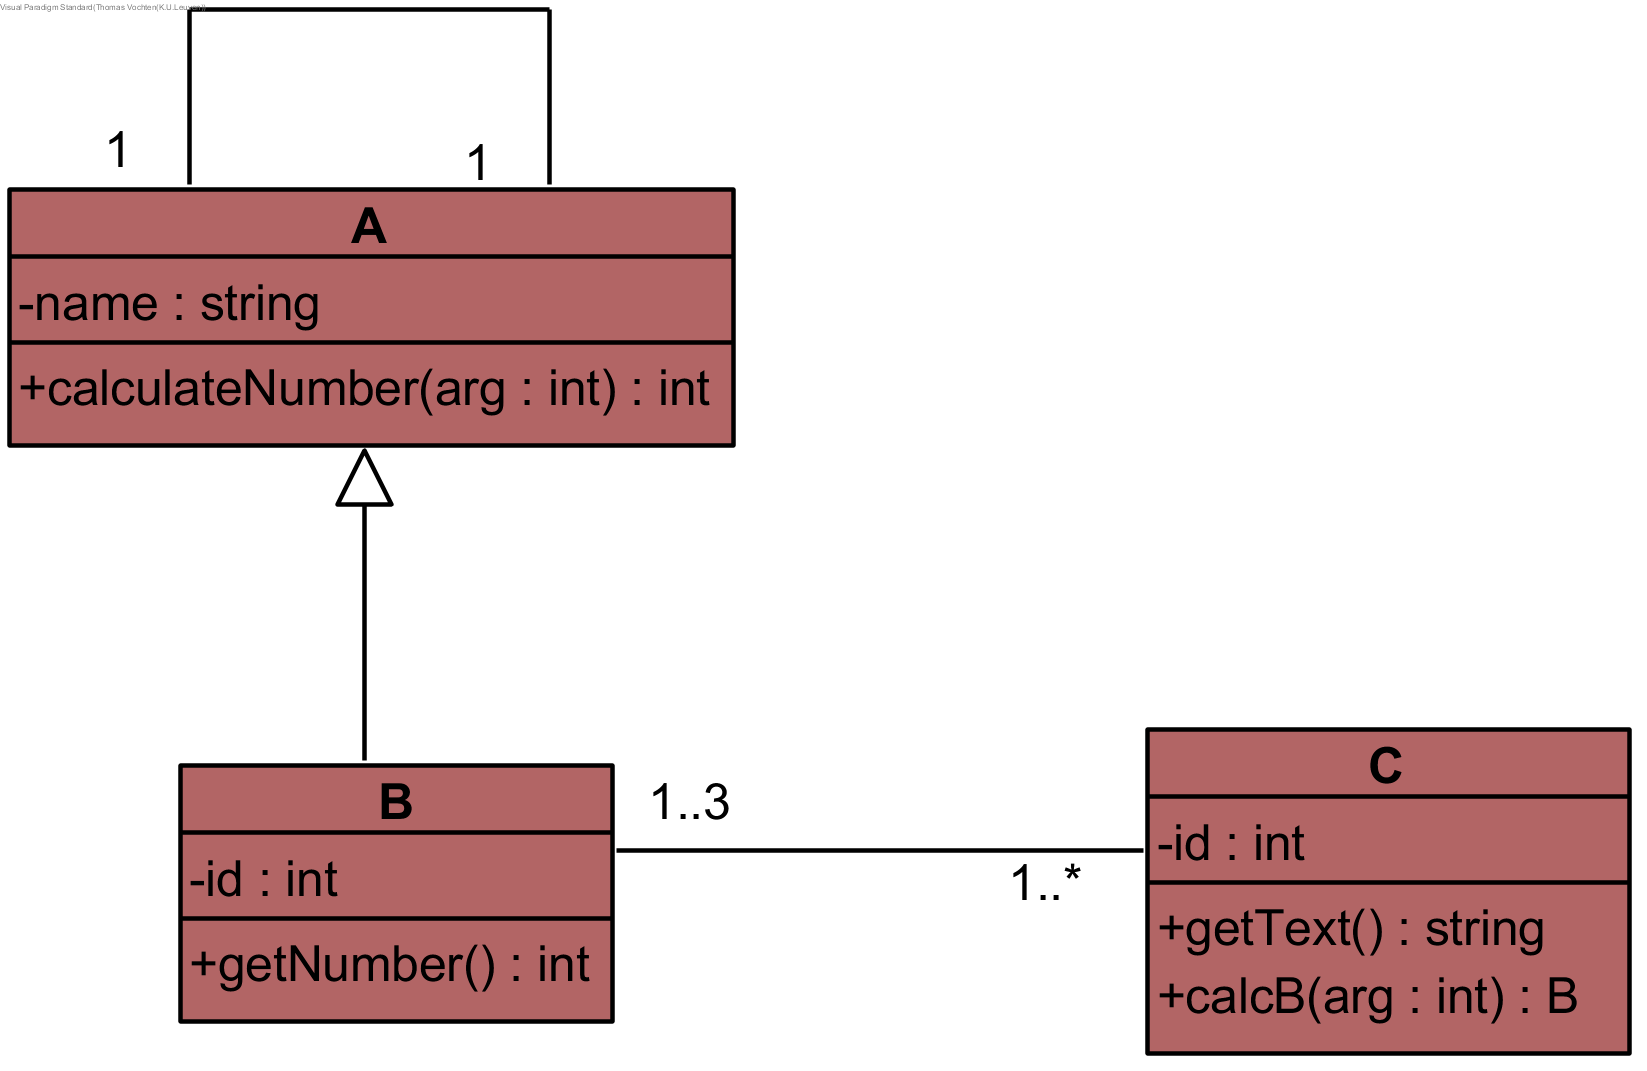
\includegraphics[width=0.6\textwidth]{chap-consistentie/voorbeeld1.png}
	\caption{Klasses, associaties en overervingsrelaties}
	\label{fig:voorbeeld1}
\end{figure}

\begin{figure}[h]
	\centering
	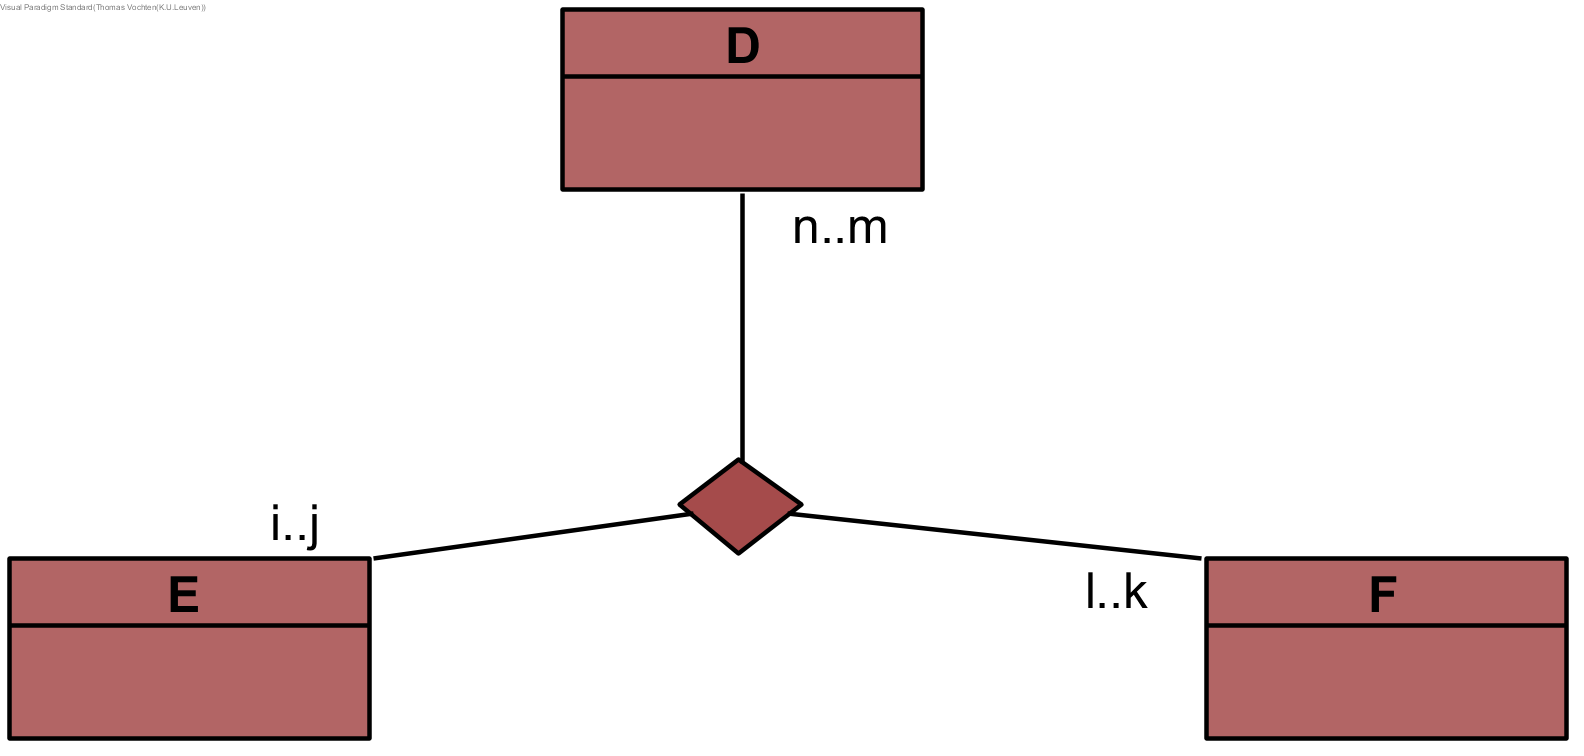
\includegraphics[width=0.6\textwidth]{chap-consistentie/voorbeeld2.png}
	\caption{Meervoudige associaties}
	\label{fig:voorbeeld2}
\end{figure}

\subsection{Klasse}

Klassediagrammen beschrijven de structuur van een object in het gemodelleerde probleemdomein. Die structuur bestaat uit discrete stukken informatie die het object bevat of kan bevatten, de bewerkingen die beschikbaar zijn voor een object, en een beschrijving van hoe men het object in verband kan brengen met andere objecten uit het probleemdomein. \textbf{Klasses} bepalen hoe die structuur eruit ziet voor een object. We zeggen dat een object een \textbf{instantie} is van een klasse als de toestand van en bewerkingen beschikbaar op dat object overeenkomen met die klasse. Dit concept defini\"eren we preciezer later in deze sectie.

Een klasse bestaat uit de volgende elementen:

\begin{itemize}
	\item Elke klasse heeft een unieke \textbf{naam} binnen eenzelfde klassediagram.
	\item \textbf{Attribuut}: De toestand van een klasse bestaat uit de combinatie van zijn attributen. Elk attribuut heeft een naam en een type. De type van een attribuut kan zowel een primitief type zijn zoals \textit{int} of \textit{string} of een andere klasse uit het diagram. Klasse \textit{A} in figuur \ref{fig:voorbeeld1} heeft \textit{name} als attribuut met als type \textit{string}. Een attribuut heeft ook een multipliciteit, genoteerd als $n..m$ waarvoor $n,m \in \mathbb{N}$ en $n \leq m$. Dit betekent dat een attribuut minimaal $n$ verschillende waarden heeft en maximaal $m$ verschillende waarden. In de plaats van een bovengrens kan er ook $*$ staan, wat betekent dat een attribuut een arbitrair aantal aan verschillende waarden kan hebben. Indien de ondergrens 0 is, kan het zijn dat er geen waarde bestaat voor die attribuut. Als het diagram geen multipliciteit specificeert voor een attribuut, dan geldt standaard dat de multipliciteit $1..1$ is. In figuur \ref{fig:voorbeeld1} heeft het attribuut \textit{id} van klasse \textit{B} een multipliciteit van $1..2$.
	\item \textbf{Operatie}: De operaties van een klasse duiden de beschikbare bewerkingen op een klasse aan. De definitie van een operatie bestaat uit een naam, mogelijks een lijst van argumenten samen met hun types, en het type van het resultaat. Het resultaattype is ofwel een primitief type, een andere klasse uit het diagram, of \textit{void}, wat betekent dat de operatie geen resultaat heeft. Klasse \textit{C} in figuur \ref{fig:voorbeeld1} heeft een operatie met als naam \textit{getB}, \'e\'en argument \textit{index} met type \textit{int}, en met als resultaattype de klasse \textit{B}.
\end{itemize}

\subsection{Overerving}\label{sec:semantics-gen}

Klassediagrammen laten toe om directe overervingsrelaties te defini\"eren tussen klasses. Het diagram in figuur \ref{fig:voorbeeld1} stelt dat \textit{A} een directe superklasse is van \textit{B}. Klasses kunnen de directe superklasse zijn van meerdere klasses en klasses kunnen de directe subklasse zijn van meerdere klasses. Dit betekent dat klassediagrammen \textbf{meervoudige overerving} toestaan. Klassehi\"erarchie\"en worden gedefinieerd door de transitieve sluiting over de directe overervingsrelaties die aanwezig zijn in een diagram.

We kunnen nu volledig het concept van \textbf{instantie} defini\"eren. Een instantie is een object dat beantwoordt aan de structuur opgelegd door een klasse. Die structuur bestaat uit de attributen en operaties gedefinieerd voor de klasse.

De \textbf{instantiatie} van een klasse is de verzameling van alle instanties van die klasse.

Een object kan een instantie zijn van meerdere klasses. In de eerste plaats is een object een directe instantie van een bepaalde klasse. Als die klasse deel uitmaakt van een klassehi\"erarchie, betekent dit dat het object een indirecte instantie is van alle superklasses van de klasse. Beschouw het diagram in figuur \ref{fig:multi-inheritance}. Het duidt directe overervingsrelaties aan door pijlen met een leeg hoofd. De klasse van waaruit de pijl vertrekt is de subklasse terwijl de klasse waarnaar de pijl wijst de superklasse is.

Een klasse kan betrokken zijn bij meerdere directe overervingsrelaties. De klasse kan een superklasse zijn van meerdere klasses. De klasse kan ook de subklasse zijn van meerdere klasses. Dit drukt meervoudige overerving uit.

In figuur \ref{fig:multi-inheritance} is klasse \textit{Z} een subklasse van klasse \textit{Y}. Door meervoudige overerving is klasse \textit{Y} een subklasse van klasses \textit{X} en \textit{O}. De transitieve sluiting over directe overervingsrelaties betekent dat directe instanties van klasse \textit{Z} ook instanties zijn van de klasses \textit{X} en \textit{O}.

UML gebruikt meervoudige overerving om \textbf{meervoudige classificatie}\cite{RumbaughJames2005Tuml} te defini\"eren. Dit laat toe dat een object een directe instantie is van meer dan \'e\'en klasse zonder dat de klasses noodzakelijk met elkaar in verband staan in een klassehi\"erarchie. Stel dat een object \textit{x} een directe instantie is van klasses \textit{H} en \textit{I}. Dit betekent dat \textit{x} feitelijk een directe instantie is van een impliciet gedefinieerde klasse \textit{J} dat zelf geen attributen of operaties definieert en een subklasse is van klasses \textit{H} en \textit{I}. De meeste objectgerichte programmeertalen implementeren meervoudige classificatie echter niet, en deze masterproef beschouwt het verder niet.

\begin{figure}
	\centering
	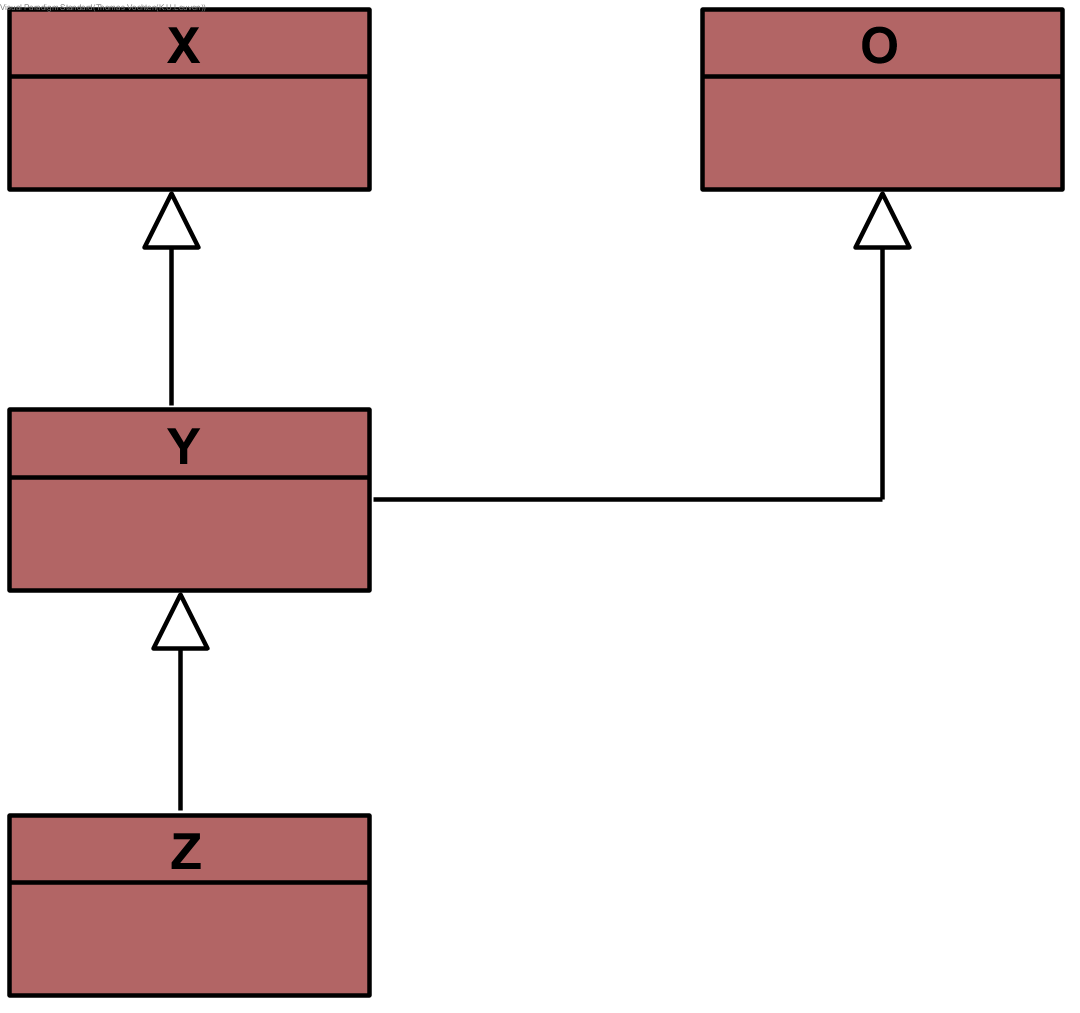
\includegraphics[width=0.5\textwidth]{chap-consistentie/voorbeeld6.png}
	\caption{Voorbeeld van meervoudige overerving}
	\label{fig:multi-inheritance}
\end{figure}

Subklasses erven alle attributen en operaties van al hun superklasses.

De specificatie van klassediagrammen stelt dat in een klassehi\"erarchie een attribuut met een bepaalde signatuur, bestaande uit zijn naam, type en multipliciteit, maar \'e\'enmaal mag gedefinieerd worden. Verder mag een operatie met een bepaalde signatuur, zijnde haar naam, lijst van parameters met hun bijhorende type, en resultaattype maar eenmaal gedefinieerd worden in deze klassehi\"erarchie, tenzij een subklasse de operatie met die signatuur herdefinieert. Dit noemt men \textit{\textbf{overriding}}. Doorgaans doet men dit om aan te geven dat een subklasse de implementatie van een bepaalde methode anders invult. De specificatie van UML\cite{OMG-UML} stelt dat bij \textit{overriding} de ontwerper zelf moet beslissen of \textbf{covariantie}, \textbf{contravariantie} of \textbf{invariantie} voor de types van de parameters en resultaat van een operatie geldt. Covariantie betekent dat een type vervangen mag worden door een subtype. Contravariantie betekent dat een type vervangen mag worden door een supertype. Invariantie betekent dat een type niet mag veranderen. Elk van deze vormen van variantie kan gelden voor parametertypes en resultaattypes.

Als een klasse deel uitmaakt van meerdere klassehi\"erarchie\"en, mag die klasse maar een definitie van een operatie van een bepaalde signatuur overerven van ten hoogste \'e\'en klassehi\"erarchie. Als een klasse een operatie van een bepaalde signatuur zelf herdefinieert, blijft het diagram wel geldig als die klasse anders meer dan \'e\'en definitie van een operatie van dezelfde signatuur zou overerven.

\subsection{Associatie}

Een associatie relateert een object aan \'e\'en of meerdere andere objecten van ofwel dezelfde klasse ofwel een andere klasse. Een associatie is ofwel binair ofwel meervoudig. We bespreken deze twee apart.

\subsubsection{Binaire associatie}\label{sec:bin-assoc}

Een binaire associatie relateert een object van een klasse aan objecten van ofwel dezelfde klasse ofwel een andere klasse. In figuur \ref{fig:voorbeeld1} relateert de associatie \textit{B}---\textit{C} objecten van klasse \textit{B} aan objecten van klasse \textit{C}, terwijl de associatie \textit{A}---\textit{A} objecten van klasse A relateert aan andere objecten van klasse \textit{A}. Er wordt niet uitgesloten dat een object van klasse \textit{A} gerelateerd wordt aan zichzelf.

Elk uiteinde van een associatie is onderhevig aan een multipliciteit, genoteerd als $n..m$ met $n,m \in \mathbb{N}$ en $n \leq m$ of $n..*$ met $n \in \mathbb{N}$. Beschouw de associatie \textit{B}---\textit{C} in figuur \ref{fig:voorbeeld1}. Een object van klasse \textit{B} moet gerelateerd zijn aan minimaal \'e\'en object van klasse \textit{C}. Er is geen bovengrens op de hoeveelheid objecten van klasse \textit{C} waaraan een object van klasse \textit{B} gerelateerd is. Een object van klasse \textit{C} moet gerelateerd zijn aan minimaal \'e\'en object van klasse \textit{B} en maximaal drie objecten van klasse \textit{B}.

De multipliciteiten op de associatie \textit{A}---\textit{A} impliceren dat elk object van klasse \textit{A} moet gerelateerd zijn aan exact \'e\'en object van klasse \textit{A}, zij het zichzelf of een ander object.

In deze masterproef beschouwen we alleen bidirectionele associaties. Dit betekent dat beide uiteindes van een associatie \textbf{navigeerbaar} zijn. Gegeven een object kan men navigatie over een associatie naar het andere uiteinde uitvoeren, wat mogelijks een object of een verzameling van objecten als resultaat heeft. Wat dit concreet betekent, hangt af van de grenzen van de multipliciteit op het uiteinde aan de andere kant in de associatie:

\begin{itemize}
	\item De multipliciteit is $1..1$: Navigatie resulteert in het unieke object waaraan het object gerelateerd is.
	\item De multipliciteit is $0..1$: Het kan zijn dat navigatie geen resultaat geeft omdat er geen gerelateerd object aan het andere uiteinde bestaat. In het andere geval heeft navigatie het gerelateerd object als resultaat.
	\item De multipliciteit is $1..n$ waarbij $n > 1$ of $1..*$: Navigatie resulteert in een verzameling dat alle gerelateerde objecten bevat als lid. Als de bovengrens $n$ is, is de maximale cardinaliteit van de verzameling $n$. Als de bovengrens $*$ is, heeft de verzameling een arbitrair grote cardinaliteit.
	\item De multipliciteit is $0..n$ waarbij $n > 0$ of $0..*$: Zoals hierboven, maar de resulterende verzameling kan leeg zijn.
\end{itemize}

\subsubsection{Meervoudige associatie}\label{sec:nary-assoc}

Er kunnen associaties bestaan tussen meer dan twee klasses tegelijk. Het diagram in figuur \ref{fig:voorbeeld2} bevat een voorbeeld van een ternaire associatie die objecten van de klasses \textit{D}, \textit{E} en \textit{F} aan elkaar relateert. We illustreren de semantiek die de specificatie van UML-klassediagrammen\cite{OMG-UML} definieert voor meervoudige associaties aan de hand van figuur \ref{fig:voorbeeld2}:

\begin{itemize}
	\item Voor elk tupel $(d,e)$ waar $d \in D, e \in E$ geldt dat minimaal $l$ objecten van klasse \textit{F} gerelateerd zijn aan het tupel en maximaal $k$ objecten van klasse \textit{F}.
	\item Voor elk tupel $(e,f)$ waar $e \in E, f \in F$ geldt dat minimaal $n$ objecten van klasse \textit{D} gerelateerd zijn aan het tupel en maximaal $m$ objecten van klasse \textit{D}.
	\item Voor elk tupel $(f,d)$ waar $f \in F, d \in D$ geldt dat minimaal $i$ objecten van klasse \textit{E} gerelateerd zijn aan het tupel en maximaal $j$ objecten van klasse \textit{D}.
\end{itemize}

Indien de ondergrens voor de multipliciteit van een uiteinde $0$ is, is het mogelijk dat een tupel geen gerelateerd object heeft. Indien de bovengrens $*$ is, is er een arbitrair aantal aan gerelateerde objecten voor een tupel.

De semantiek voor ternaire associaties opgesteld aan de hand van figuur \ref{fig:voorbeeld2} is eenvoudig te veralgemenen voor meervoudige associaties van arbitraire ariteit.

Merk op dat, als in figuur \ref{fig:voorbeeld2} $i$ gelijk is aan 1, deze semantiek impliceert dat voor alle mogelijke tupels $(d,e)$ waar $d \in D, e \in E$ er minstens \'e\'en gerelateerd object van klasse \textit{F} moet bestaan. Daarom is het gebruikelijk om de ondergrenzen voor alle uiteindes gelijk te stellen aan 0.

Ook meervoudige associaties zijn navigeerbaar. Voor associaties met een ariteit van $n$ heeft navigatie nu een tupel met ariteit $(n-1)$ als invoer. De $(n-1)$ elementen van het tupel bestaan uit objecten van de gerelateerde klasse horend bij elk uiteinde van de associatie waarbij \'e\'en uiteinde wordt uitgesloten. Er wordt genavigeerd naar het uiteinde die uitgesloten werd uit het tupel. De concrete betekenis van navigatie is analoog aan die voor binaire associaties.

\subsubsection{Het verband tussen associaties en overerving}

Subklasses nemen deel aan alle associaties gedefinieerd voor alle superklasses. Beschouw figuur \ref{fig:assoc-hier}. De klasse \textit{N} neemt deel aan zowel de associatie \textit{L}---\textit{M} als de associatie \textit{N}---\textit{O}. Het is niet zo dat een tupel dat behoort tot de associatie \textit{N}---\textit{O} behoort tot de associatie \textit{L}---\textit{M}. Associaties die een subklasse overerft en associaties die direct zijn gedefinieerd voor een subklasse zijn onafhankelijk van elkaar.

UML laat wel toe dat de ontwerper een associatie specialiseert\cite{RumbaughJames2005Tuml}. Beschouw figuur \ref{fig:assoc-gen}. De associatie \textit{J}---\textit{K} specialiseert de associatie \textit{H}---\textit{I}. Hierbij is het verplicht dat de klasses verbonden in de specialiserende associatie subklasses zijn van de klasses verbonden in de associatie die gespecialiseerd wordt. Figuur \ref{fig:assoc-gen} stelt dat alle tupels die behoren tot de associatie \textit{J}---\textit{K} ook behoren tot de associatie \textit{H}---\textit{I}, maar niet noodzakelijk omgekeerd.

\begin{figure}
	\centering
	\begin{subfigure}{0.4\textwidth}
		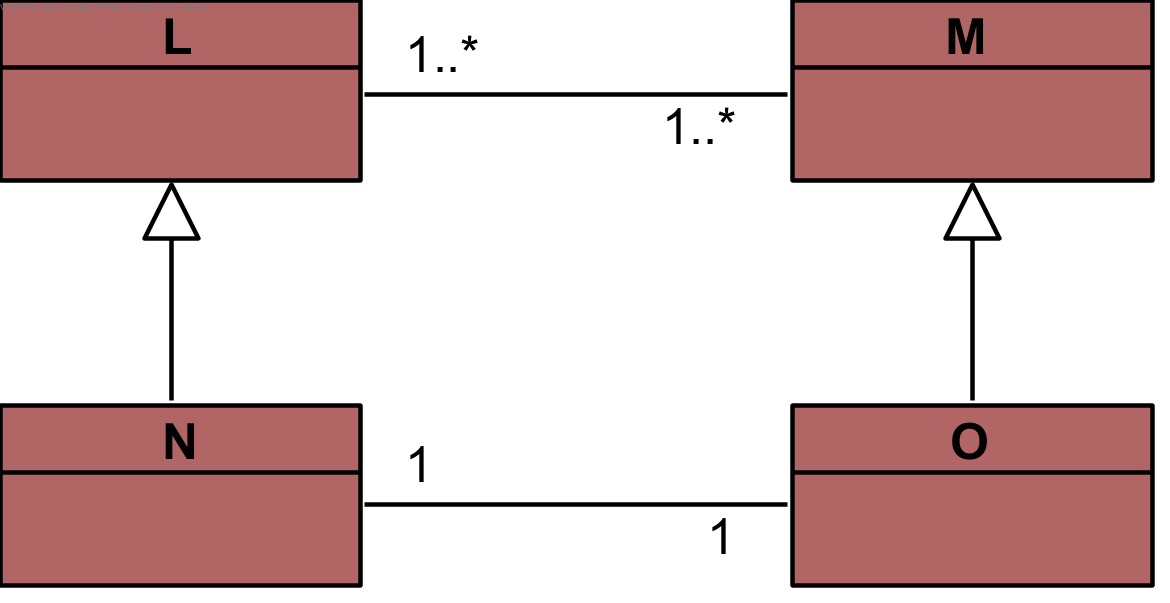
\includegraphics[width=\textwidth]{chap-consistentie/assoc-hier.png}
		\caption{Een voorbeeld van onafhankelijke associaties tussen superklasses en tussen subklasses}
		\label{fig:assoc-hier}
	\end{subfigure}
	\hfill
	\begin{subfigure}{0.4\textwidth}
		\vspace{-0.2cm}
		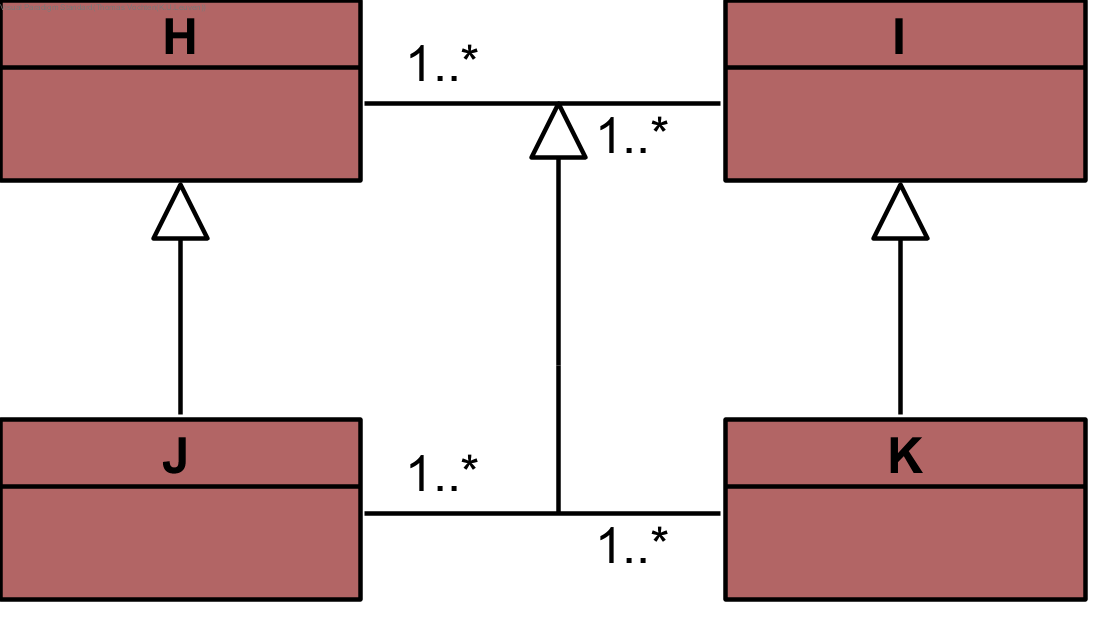
\includegraphics[width=\textwidth]{chap-consistentie/assoc-gen.png}
		\caption{Een voorbeeld van overerving van associaties}
		\label{fig:assoc-gen}
	\end{subfigure}
	\caption{Voorbeelden van associaties tussen superklasses en tussen subklasses}
	\label{fig:assoc-hier-gen}
\end{figure}

\section{Semantiek voor klassediagrammen}\label{sec:cd-semantics}

Deze sectie beschrijft een modelsemantiek voor klassediagrammen gebaseerd op de componenten genoemd in sectie \ref{sec:cd-components} en de eigenschappen daarvan.

Een model is een verzameling van de volgende delen:

\begin{itemize}
	\item Voor elke klasse de corresponderende instantiatie.
	\item Voor elk attribuut een verzameling van paren. Aan de linkerkant bevindt zich een instantie van de klasse waarvoor het attribuut gedefinieerd is en aan de rechterkant bevindt zich een waarde van het attribuut die hoort bij die instantie.
	\item Voor elke operatie een totale functie van $(m+1)$ argumenten, waar $m$ gelijk is aan het aantal parameters van de operatie. De functie specificeert voor elke mogelijke combinatie van instantie en invoerargumenten een uniek resultaat.
	\item Voor elke associatie een verzameling van $n$-aire tupels, waar $n$ de ariteit van de associatie.
\end{itemize}

Een model voldoet aan een klassediagram als en slechts het voldoet aan de volgende voorwaarden:

\begin{enumerate}
	\item Als een object een directe instantie is van een klasse, moet dat object ook een instantie zijn van alle superklasses.\label{rule:instance}
	\item Alle objecten moeten voor alle attributen gedefinieerd in de klasses waar het een directe instantie van is en voor alle overge\"erfde attributen zoveel verschillende waarden hebben als voorgeschreven door de multipliciteit van het attribuut. Als de ondergrens 0 is, kan het zijn dat er geen waarde aanwezig is. Enkel objecten die instanties zijn van de klasses waarvoor een bepaald attribuut gedefinieerd is, mogen waarden hebben voor dat attribuut.\label{rule:attr}
	\item Alle objecten moeten voor alle operaties gedefinieerd in de klasses waar het een directe instantie van is en voor alle overge\"erfde operaties voldoen aan de volgende voorwaarde: voor alle mogelijke combinaties van argumenten, allemaal van het juiste type, moet er een resultaat van het juiste type zijn. Enkel objecten die instanties zijn van de klasses waarvoor een bepaalde operatie gedefinieerd is mogen voorkomen als instanties waarvoor de functie die overeenkomt met de operatie combinaties van invoerargumenten en resultaat kent.\label{rule:op}
	\item Zij $n$ het aantal keren dat een klasse voorkomt in een uiteinde in een associatie. Voor alle tupels die lid zijn van de verzameling overeenkomend met de associatie moet gelden dat exact $n$ elementen lid zijn van die klasse.\label{rule:assoc-occ}
	\item Elk uiteinde van een associatie moet consistent dezelfde plek hebben in de tupels die lid zijn van de verzameling die overeenkomt met die associatie.\label{rule:assoc-con}
	\item Stel dat \textit{x} een instantie is van klasse \textit{X} die in verband staat met klasse \textit{Y} door middel van een binaire associatie. Het uiteinde \textit{Y} heeft een multipliciteit van $n..m$. Stel $A$ gelijk aan de verzameling van tupels die de invulling zijn van de associatie \textit{X}---\textit{Y}. Stel verder $B$ gelijk aan de deelverzameling van $A$ waar voor alle leden geldt dat \textit{x} voorkomt op de plaats horend bij uiteinde \textit{X}. Dan moet gelden dat $n \leq |B|$ en $|B| \leq m$. Als de bovengrens voor uiteinde \textit{Y} gelijk is aan $*$, is er geen bovengrens op $|B|$.\label{rule:assoc-mult}
	\item De verzameling van tupels die overeenkomt met een meervoudige associatie moet voldoen aan de semantiek voor meervoudige associaties beschreven in sectie \ref{sec:nary-assoc}.\label{rule:assoc-nary}
\end{enumerate}

Merk op dat deze voorwaarden tot gevolg hebben dat men voor alle klassediagrammen een model kan opstellen dat voldoet aan het diagram door een lege instantiatie toe te kennen aan elke klasse. We noemen dit het \textbf{triviaal model}.

We geven een voorbeeldmodel voor het diagram in figuur \ref{fig:voorbeeld1}:

\begin{itemize}
	\item Klasse \textbf{\textit{A}}: $\{a; b1; b2; b3\}$
	\item Klasse \textbf{\textit{B}}: $\{b1; b2; b3\}$
	\item Klasse \textbf{\textit{C}}: $\{c\}$
	\item Attribuut \textbf{\textit{name}} in \textbf{\textit{A}}: $\{(a,``a''); (b1,``b1''); (b2,``b2''); (b3,``b3'')\}$
	\item Attribuut \textbf{\textit{id}} in \textbf{\textit{B}}: $\{(b1,1);(b2,2);(b3,3)\}$
	\item Attribuut \textbf{\textit{id}} in \textbf{\textit{C}}: $\{(c,1)\}$
	\item Operatie \textbf{\textit{calculateNumber} in \textbf{\textit{A}}: $\{(a,n)\rightarrow{}n\}$} voor alle instanties \textit{a} van \textit{A} en voor alle $n \in \mathbb{N}$
	\item Operatie \textbf{\textit{getNumber}} in \textbf{\textit{B}}: $\{b1\rightarrow{}1; b2\rightarrow{}2; b3\rightarrow{}3\}$
	\item Operatie \textbf{\textit{getText}} in \textbf{\textit{C}}: $\{c\rightarrow{}``foo''\}$
	\item Operatie \textbf{\textit{calcB}} in \textbf{\textit{C}}: $\{(c,n)\rightarrow{}b1\}$ voor alle $n \in \mathbb{N}$
	\item Associatie \textbf{\textit{A}---\textit{A}}: $\{(a, a); (b1, b1); (b2, b2); (b3, b3)\}$
	\item Associatie \textbf{\textit{B}---\textit{C}}: $\{(b1,c); (b2,c); (b3,c)\}$
\end{itemize}

\subsection{Consistentie van klassediagrammen}

We nemen de definities voor consistentie over van Daniela Berardi et al.\cite{BerardiDaniela2005RoUc}.

\begin{definition}
Een klassediagram is consistent als en slechts als er een eindig model bestaat waarvoor minstens \'e\'en klasse minstens \'e\'en instantie bevat.
\end{definition}\label{def:diagram-consistency}

\begin{definition}
Een klasse in een klassediagram is consistent als en slechts als er een eindig model bestaat waarvoor de klasse minstens \'e\'en instantie bevat.
\end{definition}

Definitie 1 sluit het triviaal model uit.

Als gevolg van de eerder gedefinieerde semantiek voor de beschikbare componenten voor klassediagrammen in deze masterproef kan een klassediagram of een klasse inconsistent zijn ten gevolge van de aanwezige associaties en overervingsrelaties. We illustreren hoe dit kan gebeuren aan de hand van figuren \ref{fig:incon-assoc-simple}, \ref{fig:incon-assoc-multi}, \ref{fig:incon-gen-assoc} en \ref{fig:incon-assoc-spec}.

\begin{figure}
	%\vspace*{-0.5cm}
	\hspace{-3cm}
	\centering
	\begin{subfigure}[b]{0.3\textwidth}
		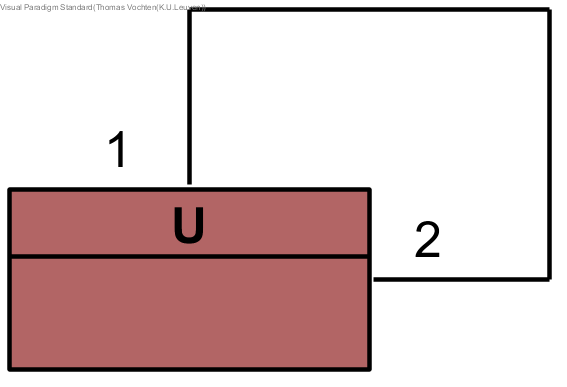
\includegraphics[width=0.6\textwidth]{chap-consistentie/voorbeeld3.png}
		\caption{}
		\label{fig:incon-assoc-simple}
	\end{subfigure}%
	\begin{subfigure}[b]{0.3\textwidth}
		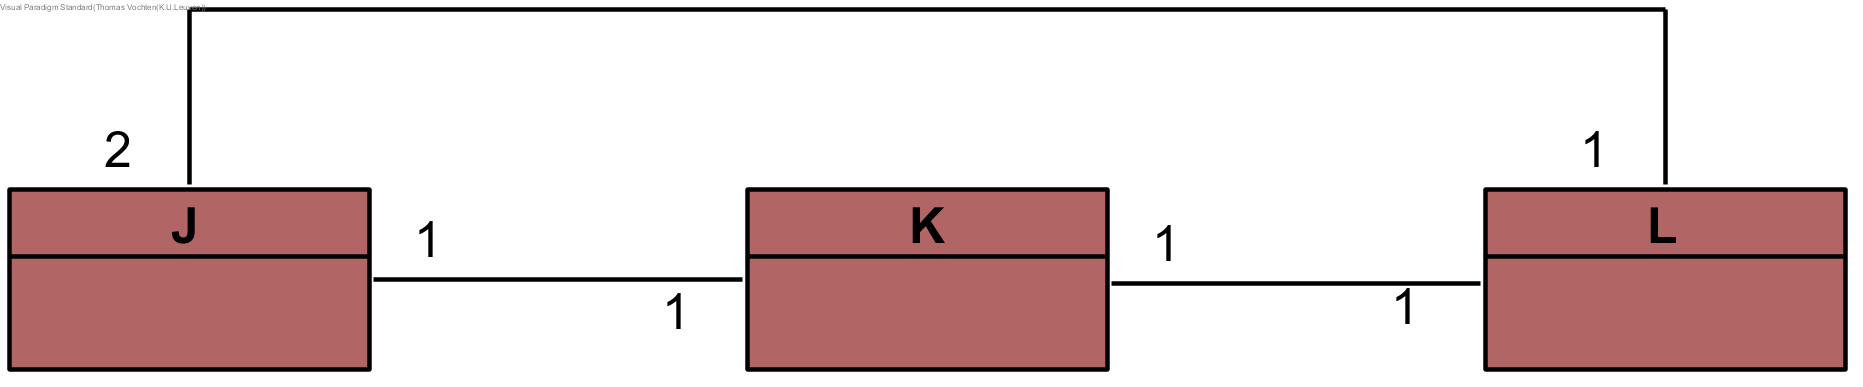
\includegraphics[width=2\textwidth]{chap-consistentie/voorbeeld4.png}
		\caption{}
		\label{fig:incon-assoc-multi}
	\end{subfigure}
	\caption{Voorbeelden van oneindige modellen ten gevolge van associaties}
	\label{fig:incon-assoc}
\end{figure}

\begin{figure}
	\centering
	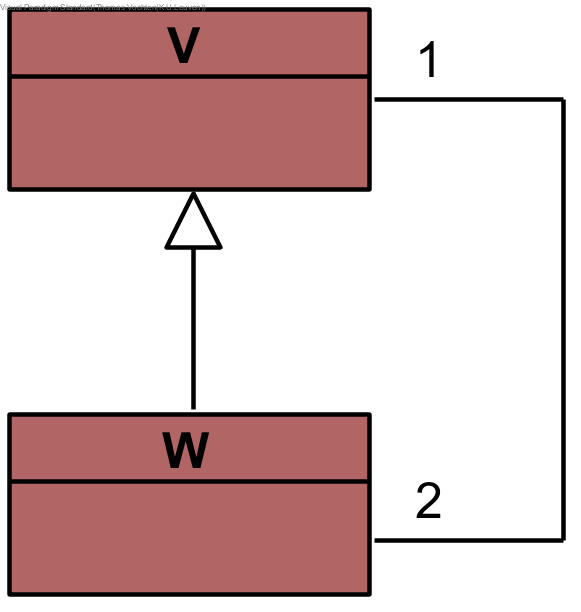
\includegraphics[width=0.175\textwidth]{chap-consistentie/voorbeeld5.png}
	\caption{Voorbeeld van oneindige modellen ten gevolge van een overervingsrelatie en associatie}
	\label{fig:incon-gen-assoc}
\end{figure}

\begin{figure}
	\centering
	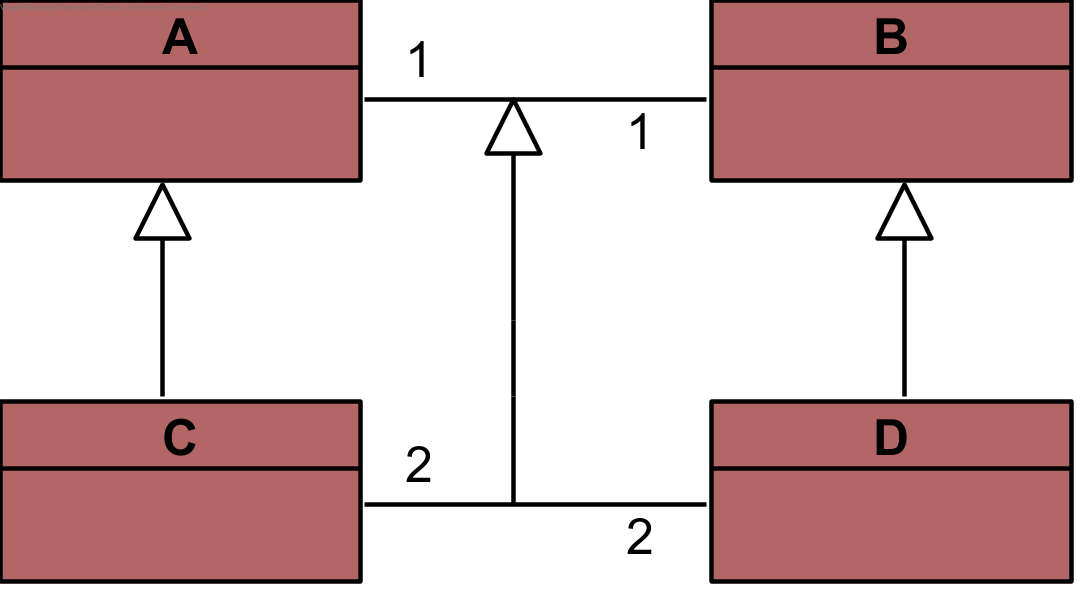
\includegraphics[width=0.30\textwidth]{chap-consistentie/assoc-incon.png}
	\caption{Voorbeeld van lege klasses ten gevolge van een gespecialiseerde associatie}
	\label{fig:incon-assoc-spec}
\end{figure}

Beschouw het diagram in figuur \ref{fig:incon-assoc-simple}. Stel dat de klasse \textit{U} twee instanties \textit{u1} en \textit{u2} bevat. We proberen de associatie in te vullen als volgt: $\{(u1, u1); (u1, u2)\}$. Om \textit{u2} twee gerelateerde objecten aan de rechterkant te geven, zouden we allereerst $(u2, u1)$ moeten toevoegen, maar dit zou ingaan tegen de multipliciteit van 1 aan de linkerkant voor \textit{u1}. Voor een gelijkaardige reden kan $(u2, u2)$ ook niet toegevoegd worden. Zo wordt er afgedwongen dat er twee extra instanties moeten toegevoegd worden: \textit{u3} en \textit{u4}. Zo kunnen we $(u2, u3)$ en $(u2, u4)$ toevoegen. Wanneer we \textit{u3} en \textit{u4} allebei twee gerelateerde objecten aan de rechterkant willen geven, doet zich echter een gelijkaardig probleem als voor \textit{u2} voor waardoor de toevoeging van \textit{u3} en \textit{u4} nodig was in de eerste plaats. Dit zorgt ervoor dat een geldig niet-leeg model voor dit diagram oneindig groot zou moeten zijn en dat de klasse \textit{U} inconsistent is.

Beschouw het diagram in figuur \ref{fig:incon-assoc-multi}. De associaties \textit{J}---\textit{K} en \textit{K}---\textit{L} hebben tot gevolg dat \textit{J}, \textit{K} en \textit{L} exact even veel instanties moeten bevatten. De associatie \textit{J}---\textit{L} stelt echter dat alle instanties van klasse \textit{L} in verband moeten staan met twee instanties van klasse \textit{J}. Dit zorgt ook voor oneindig grote niet-lege modellen en dus inconsistentie van het diagram.

Beschouw het diagram in figuur \ref{fig:incon-gen-assoc}. Stel dat klasse \textit{V} als directe instantie \textit{v} heeft en klasse \textit{W} als directe instanties \textit{w1} en \textit{w2}. We stellen $\{(v, w1); (v, w2)\}$. \textit{w1} en \textit{w2} zijn echter ook instanties van klasse \textit{V}, waardoor er vier nieuwe objecten nodig zijn om de associatie voor beide objecten te vervullen. Het probleem zet zich voor de vier objecten verder. Dit zorgt weer voor oneindig grote niet-lege modellen en inconsistentie van het diagram.

Beschouw het diagram in figuur \ref{fig:incon-assoc-spec}. Een instantie van klasse \textit{C} moet gerelateerd zijn aan twee instanties van klasse \textit{D}. Deze tupels moeten ook lid zijn van de associatie \textit{A}---\textit{B}, maar de multipliciteiten op die associatie beletten dat beide tupels tegelijkertijd lid zijn. De voorwaarde dat alle tupels in de associatie \textit{C}---\textit{D} lid moeten zijn van de associatie \textit{A}---\textit{B} is dus geschonden. Dit zorgt ervoor dat de instantiatie van \textit{C} noodzakelijk leeg is. \textit{C} is dus inconsistent. Een gelijkaardige redenering geldt voor klasse \textit{D}.

\section{Voorstellingswijze van klassediagrammen in FO($\cdot$) volgens de voorgestelde semantiek}\label{sec:cd-rep-cons}

Deze sectie beschrijft hoe we klassediagrammen voorstellen in FO($\cdot$). Daarvoor willen we een specifieke vorm van logische theorie automatisch laten genereren. In deze theorie\"en staan objecten centraal. 

Het merendeel van het werk in deze sectie bestaat erin om de methode om klassediagrammen te vertalen naar eerste-orde-predicatenlogica ge\"introduceerd in Daniela Berardi et al.\cite{BerardiDaniela2005RoUc} aan te passen om gebruik te maken van logische types zoals gedefinieerd in FO($\cdot$).

Aan de hand van het voorbeeld in figuur \ref{fig:diagram-voorbeeld} illustreren we welke regels we gebruiken om een theorie op te bouwen. Dit diagram stelt een spel voor waar personages zich bevinden op een rechthoekig veld. Personages hebben bepaalde eigenschappen in de vorm van numerieke parameters, kunnen voorwerpen bezitten en kunnen elkaar aanvallen met wapens.

\begin{figure}[h]
	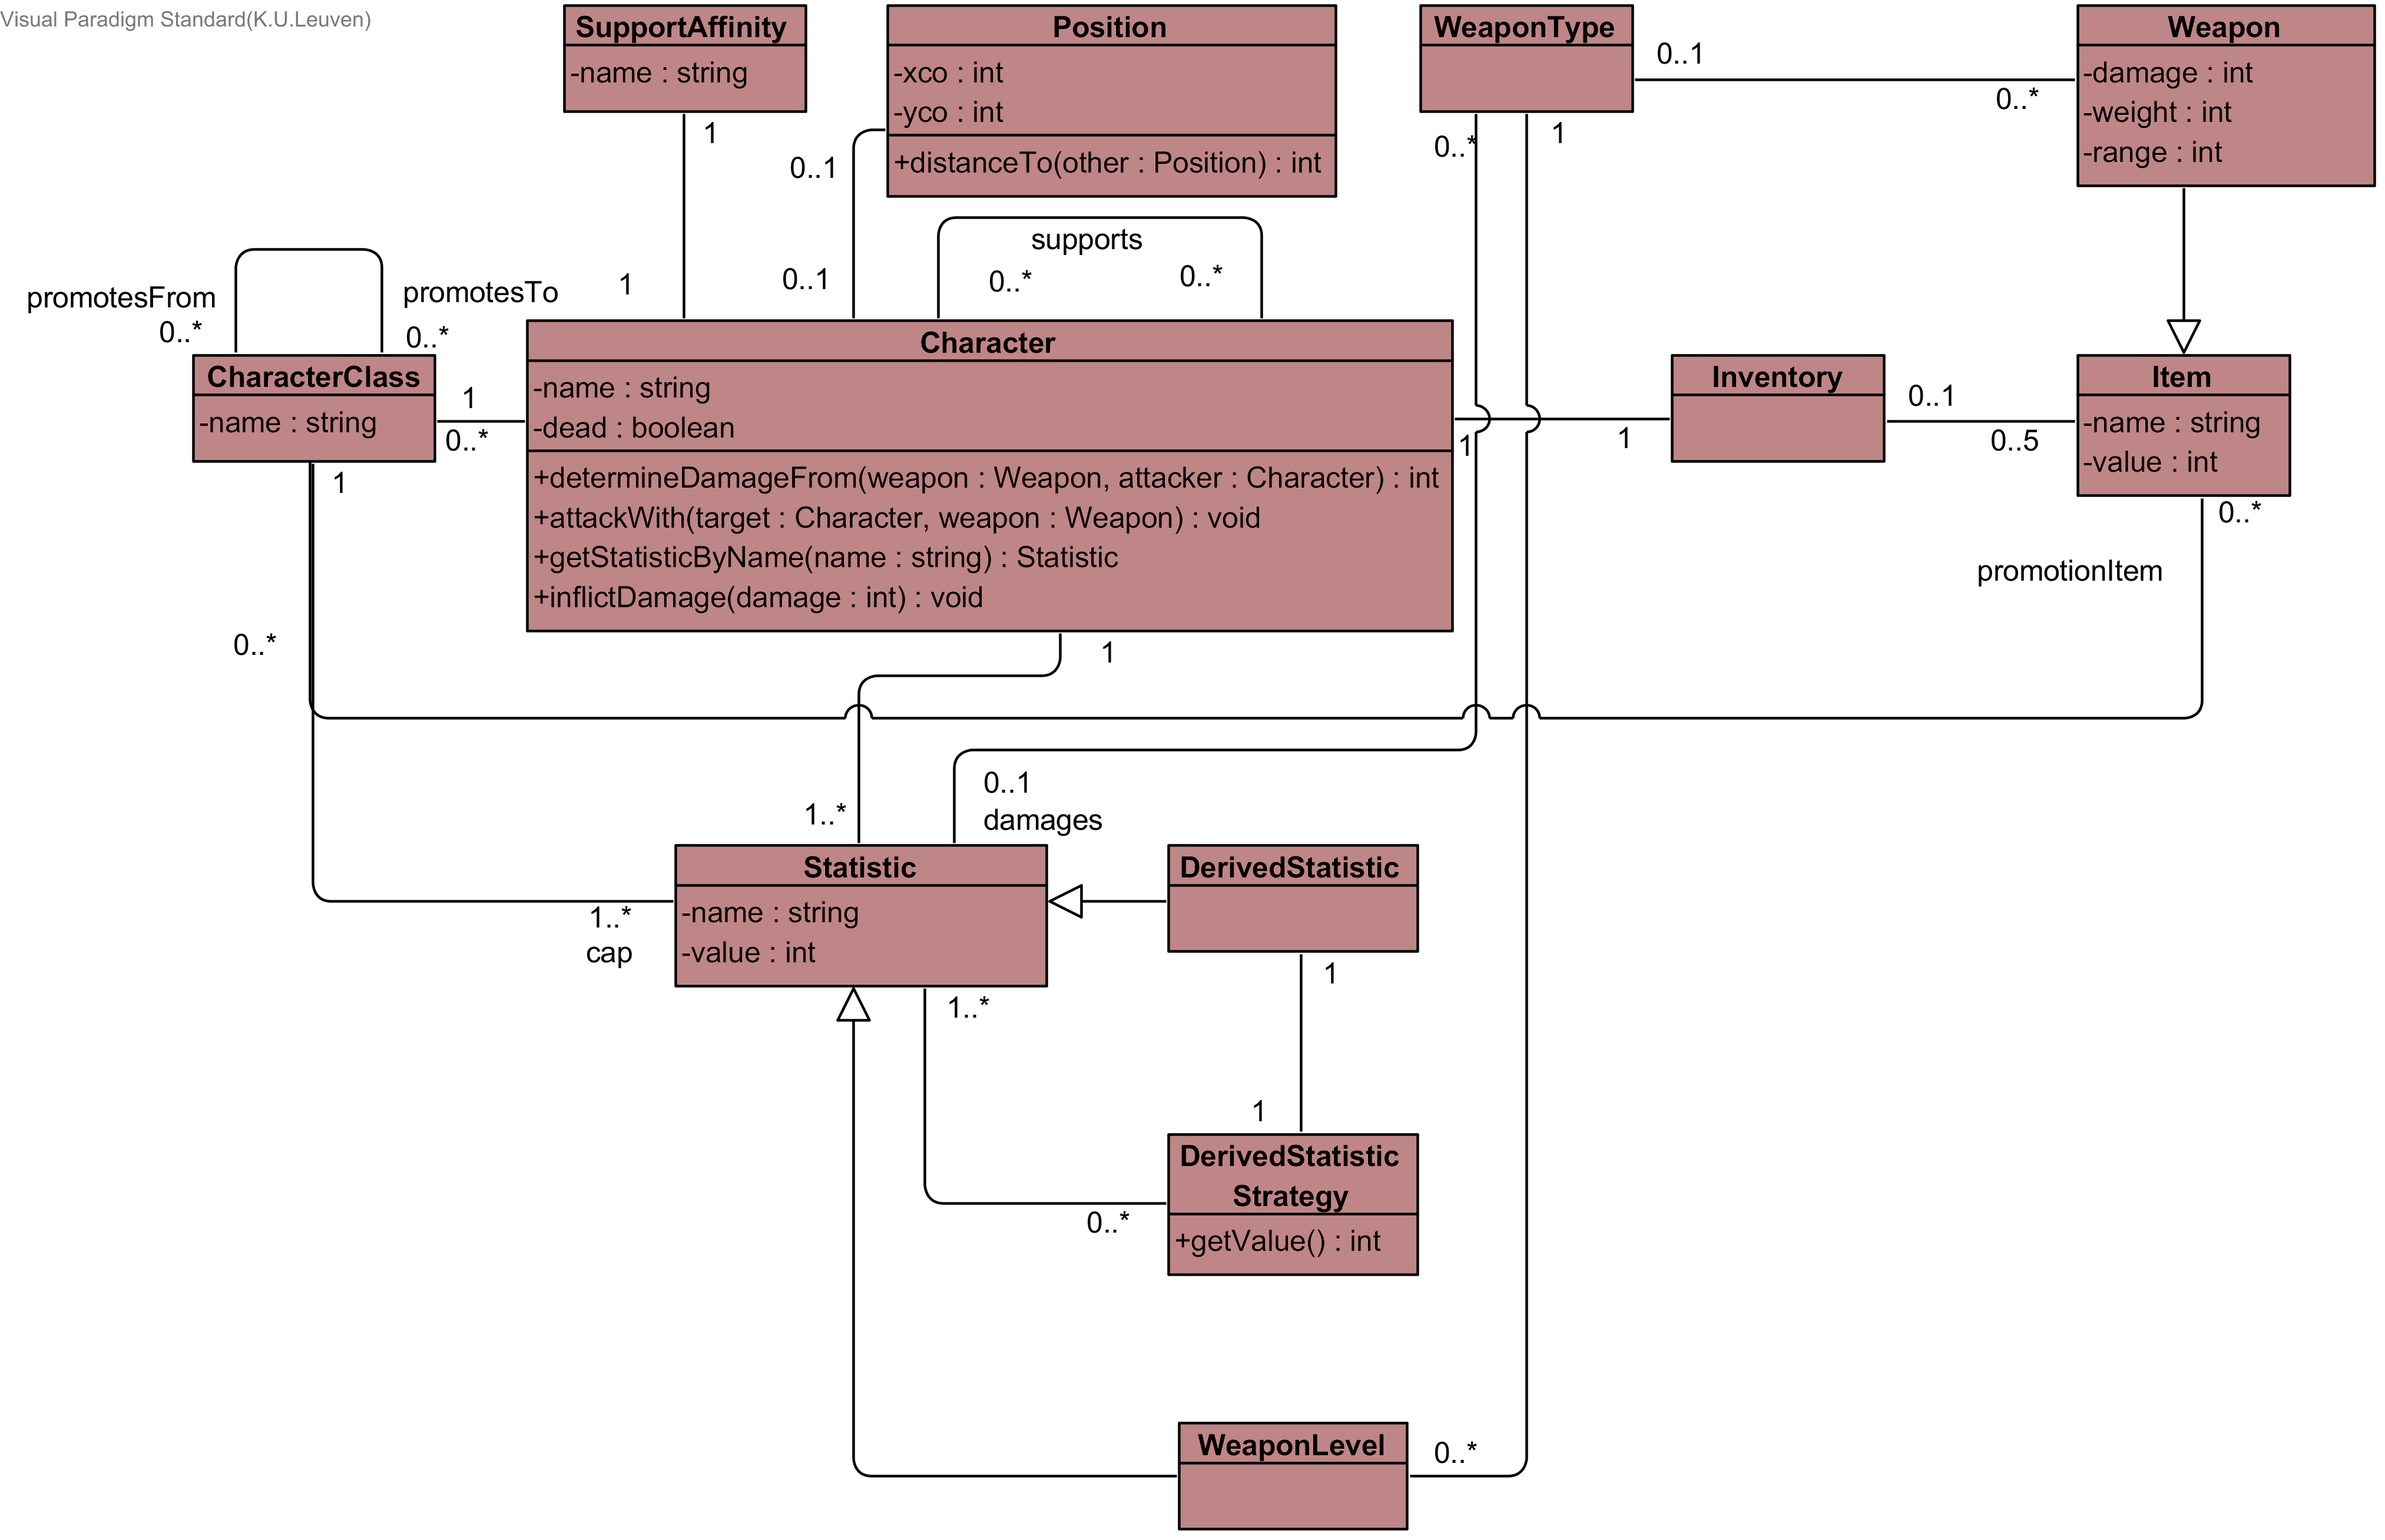
\includegraphics[width=0.95\textwidth]{chap-consistentie/diagram-voorbeeld.png}
	\caption{Leidend voorbeeld van een klassediagram}
	\label{fig:diagram-voorbeeld}
\end{figure}

We willen uitdrukken welke \textbf{klasses} er bestaan in het diagram, welke \textbf{attributen} en \textbf{operaties} elke klasse bevat, welke \textbf{associaties} er bestaan tussen de verscheidene klasses en welke \textbf{klassehi\"erarchie\"en} er bestaan.

\subsection{Logische types voor objecten}
We moeten een manier hebben om objecten te benoemen in een theorie en te specificeren tot welke klasse die objecten behoren. Voor beide van deze noden zijn logische types geschikt. We voegen voor elke klasse een logisch type toe aan het vocabularium. Er is bijvoorbeeld een logisch type \textit{Character} en een logisch type \textit{Position}. Op deze manier garanderen we voorwaarde \ref{rule:instance} voor modellen van een klassediagram.

\subsection{Voorstellen van attributen}
Voor elk attribuut voegen we een binair predicaat toe waarvan de naam beantwoordt aan het patroon: \textit{Klassenaamattribuutnaam}. Voor klasse \textit{Character} en attribuut \textit{name} resulteert dit dus in het predicaat \textit{Charactername/2}. Het eerste argument van dit predicaat is een \textit{Character}. Het type van het tweede argument hangt af van wat er in het diagram staat. Als het een primitief type is zoals \textit{string} of \textit{int}, zal dat ook het type zijn van het tweede predicaat. In het andere geval is het type van het tweede argument het overeenkomstig logisch type voor die klasse. Op deze manier dwingen we af dat elk argument van het predicaat van het juiste type is.
De signatuur van \textit{Charactername/2} is daarom \textit{Charactername(Character, string)}.
Voor elk attribuut wordt ook een regel omtrent multipliciteit afgeleid. Zij \textit{lowerBound} de ondergrens en \textit{upperBound} de bovengrens. Dan is de meest algemene vorm van deze regel als volgt:
	
\begin{align*}
	\forall{o1}[KlasseType](lowerBound \leq \#\{o2 [AttribuutType] : \\ Klassenaamattribuutnaam(o1,o2)\} \leq upperBound).
\end{align*}
	
waarbij \textit{lowerBound} wordt weggelaten als deze $0$ is en \textit{upperBound} wordt weggelaten als deze $*$ is. Indien beide van deze voorwaarden gelden, wordt er geen regel afgeleid betreffende de multipliciteit van het attribuut. Als $lowerBound = upperBound$, wordt deze regel in de plaats:
	
\begin{align*}
	\forall{o1}[KlasseType] \exists_{=upperBound}{o2}[AttribuutType](Klassenaamattribuutnaam(o1,o2)).
\end{align*}
	
Voor \textit{Charactername/2} wordt daarom afgeleid:
	
\begin{align*}
	\forall{o1}[Character]\exists_{=1}{x}[string](Charactername(o,x)).
\end{align*}

Met deze predicaten en de beperkingen erop garanderen we voorwaarde \ref{rule:attr} voor modellen van een klassediagram.

\subsection{Voorstellen van operaties}\label{sec:cons-method}
Voor elke operatie voegen we een functie toe dat beantwoordt aan volgend patroon: \sloppy
	 \textit{Klassenaamoperatienaam/(m+1) : ResultaatType}, waarbij $m$ het aantal argumenten dat als invoer wordt meegegeven aan de operatie en \textit{ResultaatType} het type van het resultaat, zij het een primitief type of een klasse. De signatuur ziet eruit als \textit{$Klassenaamoperatienaam(O,P_1,\ldots,P_m)\ :\ R$}, waarbij \textit{O} het logisch type overeenkomstig de klasse waarvan de operatie deel is, \textit{$P_1$} \ldots \textit{$P_m$} de logische types overeenkomstig de respectievelijke argumenten en \textit{$R$} het logisch type overeenkomstig het resultaat. Indien er geen argumenten zijn, ziet de signatuur eruit als \textit{Klassenaamoperatienaam(O) : R}. Voor \textit{determineDamageWeaponFrom(Weapon)} van \textit{Character} wordt dit dus \textit{CharacterdetermineDamageFrom(Character,Weapon) : int}.

Voor elke combinatie van object waarop de operatie wordt opgeroepen en mogelijke invoerparameters moet gelden dat er \'e\'en enkel resultaat is. Dit is triviaal het geval aangezien een functie elk element uit het domein afbeeldt op exact \'e\'en element uit het codomein.

Met deze functies garanderen we voorwaarde \ref{rule:op} voor modellen van een klassediagram.

\subsection{Voorstellen van associaties}
Voor elke associatie voegen we een predicaat toe dat beantwoordt aan volgend patroon: \textit{$ClassOneand\ldots{}andClassM/m$}, waarbij \textit{m} de ariteit van de associatie. Voor de associatie tussen \textit{Inventory} en \textit{Item} wordt dit dus \textit{InventoryandItem(Inventory,Item)}.

De multipliciteit voor elke rol moet worden uitgedrukt. Voor alle $o_l$ waarvoor $1 \leq l \leq m$ wordt een regel toegevoegd van de volgende vorm:\\

Zij $lowerBound_l$ de ondergrens en $upperBound_l$ de bovengrens:
\begin{align*}
	&\forall{c_1}[Klasse_1]\ldots\forall{c_m}[Klasse_m](lowerBound_l \leq
	\\
	&\#\{o_l[Klasse_l] : ClassOneand\ldots{}andClassM(c_1,\ldots,o_l,\ldots,c_m)\} \leq upperBound_l).
\end{align*}
	
waarbij de \textit{c} met index \textit{l} overgeslagen wordt. Indien de ondergrens gelijk is aan $0$ of de bovengrens gelijk is aan $*$ worden deze weggelaten. Als beide voorwaarden gelden, wordt voor deze \textit{l} geen regel afgeleid. Indien $lowerBound_l = upperBound_l$ wordt in de plaats afgeleid:
	
	\begin{align*}
	&\forall{c_1}[Klasse_1]\ldots\forall{c_m}[Klasse_m] \exists_{=upperbound_l}o_l[Klasse_l](ClassOneand\ldots{}andClassM\\&(c_1,\ldots,o_l,\ldots,c_m)).
	\end{align*}
	
	Voor \textit{InventoryandItem/2} worden de volgende regels afgeleid:
	
\begin{align*}
		\forall{o_2}[Item](\#\{o_1[Inventory]: InventoryandItem(o_1,o_2)\} \leq 1).
\end{align*} 
		
\begin{align*}
		\forall{o_1}[Inventory](\#\{o_2[Item]: InventoryandItem(o_1,o_2)\} \leq 5).
\end{align*}

Met deze predicaten en de beperkingen erop garanderen we voorwaardes \ref{rule:assoc-occ}, \ref{rule:assoc-con}, \ref{rule:assoc-mult} en \ref{rule:assoc-nary} voor modellen van een klassediagram.

\subsection{Voorstellen van klassehi\"erarchi\"een}\label{sec:hierarchies}
We beschrijven twee alternatieven om klassehi\"erarchie\"en voor te stellen.

\subsubsection{Subtypering van logische types}

Aangezien FO($\cdot$) een getypeerde logica is, is het eenvoudig om klassehi\"erarchie\"een voor te stellen. Als volgens het diagram klasse \textit{X} een subklasse is van klasse \textit{Y}, dan is het voldoende om in het uitvoervocabularium te noteren dat logisch type \textit{Y} een supertype is van logisch type \textit{X}. Het is mogelijk om op die manier een keten van overervingsrelaties te modelleren en zo een hi\"erarchie te verkrijgen. In IDP in het bijzonder is het mogelijk dat een logisch type een subtype is van meer dan \'e\'en type, dus kan men ook meervoudige overerving modelleren.

Op deze manier garanderen we dat alle modellen van de gegenereerde logische theorie beantwoorden aan de semantiek van overerving zoals besproken in alle voorwaardes behalve voorwaarde \ref{rule:assoc-con}.

Dit heeft echter een gevolg voor interpretaties van het logisch type overeenkomstig met een superklasse in een mogelijke structuur volgens het uitvoervocabularium. Indien klasse \textit{Z} een subklasse is van klasse \textit{X} uit de vorige paragraaf, dan moeten alle objecten die behoren tot klasse \textit{Z} ook behoren tot klasse \textit{X}, en zo ook moeten alle objecten die behoren tot klasses \textit{Z} en \textit{X} behoren tot klasse \textit{Y}. Dit leidt tot enig manueel werk om in IDP een geldige invoerstructuur voor inferentie op te geven.

\subsubsection{Een nieuw predicaat \textit{IsSupertypeOf/2}}

Het is mogelijk om automatisch de geschikte interpretaties te laten berekenen door af te stappen van een logisch type voor elke klasse en in de plaats twee nieuwe logische types te introduceren: Een algemeen logisch type voor objecten, \textit{Object}; en een \textit{constructed type}\cite{DeCatBroes2014PLaa} dat voor elke klasse in het diagram een overeenkomstig object heeft, \textit{ClassObject}.

Om lidmaatschap van een klasse uit te drukken, zijn er verder twee nieuwe predicaten nodig: \textit{RuntimeClass(ClassObject, Object)}, wat voor elk object uitdrukt van welke klasse het een directe instantie is; en \textit{StaticClass(ClassObject, Object)}, wat voor elk object uitdrukt van welke klasses het een directe of indirecte instantie is.

Er zijn ook twee predicaten nodig om overervingsrelaties tussen klasses te modelleren: \textit{IsDirectSupertypeOf(ClassObject, ClassObject)} om directe overervingsrelaties voor te stellen; en \textit{IsSupertypeOf(ClassObject, ClassObject)} dat de transitieve sluiting voor \textit{IsDirectSupertypeOf/2} voorstelt. Aangezien het in predicatenlogica onmogelijk is om een algemene voorstelling voor transitieve sluitingen uit te drukken, maken we gebruik van inductieve definities\cite{DeCatBroes2014PLaa}:

\begin{align}
\{
\nonumber &\forall{x}[ClassObject]\forall{y}[ClassObject](\mathit{IsSupertypeOf}(x,y) \leftarrow \\ &\mathit{IsDirectSupertypeOf}(x,y)).\label{def:tc1} \\
\nonumber &\forall{x}[ClassObject]\forall{y}[ClassObject](\mathit{IsSupertypeOf}(y,x) \leftarrow \\
&\exists{z}(\mathit{IsSupertypeOf(y,z)} \land \mathit{IsSupertypeOf}(z,x))).\label{def:tc2}
\}
\end{align}

\sloppy Zin \ref{def:tc1} maakt gebruik van \textit{IsDirectSupertypeOf/2} om een basisgeval voor \\ \textit{IsSupertypeOf/2} op te stellen. Zin \ref{def:tc2} bouwt dan verder de hi\"erarchie\"en op.

We maken in een tweede definitie gebruik van \textit{IsSupertypeOf/2} om \textit{StaticClass/2} in te vullen:

\begin{align*}
\{
&\forall{x}[ClassObject]\forall{o}[Object](StaticClass(x,o) \leftarrow RuntimeClass(x,o)). \\
&\forall{x}[ClassObject]\forall{y}[ClassObject]\forall{o}[Object](StaticClass(y,o) \leftarrow \\ &RuntimeClass(x,o) \land \mathit{IsSupertypeOf}(y,x)).
\}
\end{align*}

In een aparte definitie lijsten we de invulling voor \textit{IsDirectSupertype/2} gebaseerd op het diagram op. Voor het diagram in figuur \ref{fig:diagram-voorbeeld} wordt dit:

\begin{align*}
\{
&\mathit{IsDirectSupertypeOf}(Statistic,Weaponlevel) \leftarrow .\\
&\mathit{IsDirectSupertypeOf}(Statistic,DerivedStatistic) \leftarrow .\\
&\mathit{IsDirectSupertypeOf}(Item,Weapon) \leftarrow .\\
\}
\end{align*}

We hebben echter niet voor deze voorstellingswijze gekozen om twee redenen:

\begin{enumerate}
	\item Attribuutpredicaten, operatiepredicaten en associatiepredicaten zouden logisch type \textit{Object} als argumenten moeten hebben. Dit betekent dat er nieuwe regels nodig zijn die afdwingen dat die objecten van het juiste type zijn. Grotere theorie\"en leiden tot een langere rekentijd en hoger geheugengebruik bij de uitvoering van redeneertaken.
	\item De multipliciteitsregels zouden ook herschreven moeten worden om gebruik te maken van \textit{StaticClass}. Dit maakt zinnen over de hele lijn langer en zorgt ervoor dat ze moeilijker te begrijpen zijn.
\end{enumerate}

\subsubsection{Voorstellen van gespecialiseerde associaties}

Stel dat een associatie \textit{Y}---\textit{Z} een specialisatie is van de associatie \textit{W}---\textit{X}. \textit{Y} is een subklasse van \textit{W} en \textit{Z} is een subklasse van \textit{X}. Omdat we klassehi\"erarchie\"en voorstellen door subtypering van logische types, is het voldoende om een zin toe te voegen van de vorm:
 
\begin{align*}
	\forall{y}[Y]\forall{z}[Z](YandZ(y, z) \Rightarrow WandX(y, z)).
\end{align*}

Dit dwingt af dat alle tupels in de associatie \textit{Y}---\textit{Z} lid zijn van de associatie \textit{W}---\textit{X}.

Voor de associatie \textit{J}---\textit{K} in diagram \ref{fig:assoc-gen} krijgen we dus:

\begin{align*}
	\forall{j}[J]\forall{k}[K](JandK(j, k) \Rightarrow HandI(j, k)).
\end{align*}

\subsubsection{Herdefinities van attributen en operaties}

Sectie \ref{sec:semantics-gen} stelt dat een klassehi\"erarchie een attribuut met een bepaalde signatuur maar eenmaal mag defini\"eren. Verder mag een klasse een definitie van een operatie met een bepaalde signatuur overerven van slechts \'e\'en klassehi\"erarchie, tenzij de klasse de operatie herdefinieert door middel van \textit{overriding}. Voor eenvoud van implementatie controleert onze voorstellingswijze niet op herdefinities van attributen of operaties. Als een operatie wordt geherdefinieerd door \textit{overriding}, worden de oorspronkelijke operatie en de herdefinitie ervan behandeld als twee aparte operaties. Indien we toch zouden willen controleren op conflicterende definities en \textit{overriding} zouden willen modelleren, moeten we attributen en operaties \textbf{re\"ificeren}. Dit houdt in dat het vocabularium een logisch type bevat voor attributen en een logisch type voor operaties. Voor attributen moeten we dan functies defini\"eren voor elk aspect van de signatuur van het attribuut: naam, ondergrens van de multipliciteit, bovengrens van de multipliciteit en type van het attribuut. We moeten dan ook een binair predicaat defini\"eren dat voor elke klasse specificeert welke attributen ze defini\"eren. Analoog verkrijgen we voor operaties functies die de naam en resultaattype geven en een predicaat dat voor alle operaties definieert welke parameters ze hebben. Verder moet er een binair predicaat zijn dat attributen met equivalente definities met elkaar in verband brengt. Daarbij vergelijken we de attributen van een bepaalde klasse enkel met attributen van klasses die deel uitmaken van de klassehi\"erarchie\"en waar die klasse lid van is. We voegen ook zulk een predicaat toe voor operaties, met een analoge invulling. De uitvoertheorie stelt dan dat de interpretatie van het predicaat voor duplicate attributen leeg is en dat operaties enkel in verband mogen staan met elkaar als een klasse een operatie overerft van maar \'e\'en hi\"erarchie of als de subklasse de operatie herdefinieert door middel van \textit{overriding}.

\section{Het verifi\"eren van consistentie en inconsistentie}\label{sec:cons-verify}

Consistentie van een klassediagram kan aangetoond worden door, gegeven een theorie afgeleid volgens de regels beschreven in sectie \ref{sec:cd-rep-cons}, niet-lege structuren te geven als invoer voor modelexpansie. Indien een structuur uitgebreid kan worden tot een model, is consistentie bewezen.

Bijlage \ref{app:consistentie} bevat het resultaat van de vertaling volgens de regels in sectie \ref{sec:cd-rep-cons} voor diagram \ref{fig:diagram-voorbeeld}.

Als we een structuur die \'e\'en directe instantie toekent aan elke klasse opgeven voor deze theorie, breidt IDP ze uit tot een model voor de theorie. De conclusie is dus dat het diagram in figuur \ref{fig:diagram-voorbeeld} consistent is.

Analoog kan men de consistentie van een klasse controleren door invoerstructuren op te geven die minstens \'e\'en instantie toekennen aan de klasse.

Om te controleren op inconsistentie gebruiken we de functie \textit{entails(theory, theory)} aangeboden door IDP\cite{DeCatBroes2014PLaa}. Deze functie controleert of de rechtse theorie een logisch gevolg is van de linkse theorie. We laten IDP gebruik maken van SPASS\cite{SPASS}.

Eerst verifi\"eren we de inconsistentie van de klasses \textit{C} en \textit{D} in diagram \ref{fig:incon-assoc-spec}. De vraag is of de instantiaties voor die klasses noodzakelijk leeg zijn. Noem $T$ de theorie gegenereerd uit diagram \ref{fig:incon-assoc-spec} en noem de volgende theorie $T1$:

\begin{align*}
	\lnot{}\exists{c}[C](C(c)). \\
	\lnot{}\exists{d}[D](D(d)).
\end{align*}

SPASS antwoordt dat $T1$ een logisch gevolg is van $T$. Klasses \textit{C} en \textit{D} zijn dus inconsistent.

Vervolgens verifi\"eren we de inconsistentie van diagram \ref{fig:incon-assoc-simple}. Aangezien het triviaal model voldoet aan elk klassediagram, proberen we in de plaats te controleren of elk niet-leeg model oneindig groot moet zijn. Om het triviaal model uit te sluiten, voegen we eerst het volgende toe aan de gegenereerde theorie:

\begin{align*}
	\exists{a}[A](A(a)).
\end{align*}

Noem deze theorie \textit{T}. We kijken eerst of de volgende theorie een logisch gevolg is van \textit{T}:

\begin{align*}
	\#\{a [A] : A(a)\} > 2.
\end{align*}

SPASS besluit dat deze theorie een logisch gevolg is van \textit{T}. We kijken vervolgens of deze theorie een logisch gevolg is van \textit{T}:

\begin{align*}
\#\{a [A] : A(a)\} > 3.
\end{align*}

SPASS geeft echter geen besluit binnen een redelijke tijdspanne. Controleren of modellen voor theorie\"en gegenereerd volgens de regels beschreven in sectie \ref{sec:cd-rep-cons} noodzakelijk oneindig groot zijn is dus een mogelijke piste voor verder onderzoek.

\section{Controleren op kwaliteitsgebreken}\label{sec:kwaliteitsgebrek}
Deze sectie beschrijft een alternatieve voorstellingsmethode voor klassediagrammen waarmee we bepaalde soorten kwaliteitsgebreken kunnen detecteren. Waar in sectie \ref{sec:cd-rep-cons} objecten centraal stonden, doen we daar hier afstand van: we abstraheren de logische types voor klasses weg en concentreren ons in de plaats op \textit{ClassObject}, een \textit{constructed type} dat een overeenkomstig object heeft voor alle klasses in het diagram. We gebruiken het diagram in figuur \ref{fig:diagram-voorbeeld} weer als begeleidend voorbeeld. In de volgende secties overlopen we hoe we de theorie die we gebruiken voor dit probleem opbouwen.

\subsection{Gebruikte logische types en predicaten}
\sloppy Waar we in sectie \ref{sec:hierarchies} het logisch type \textit{ClassObject} en het predicaat \textit{IsSupertypeOf/2} afwezen, behouden we deze hier.

We gebruiken daar bijkomend de volgende nieuwe logische symbolen:

\begin{itemize}
	\item \textbf{\textit{BiAssoc(ClassObject,ClassObject)}}: drukt uit dat er een binaire associatie bestaat tussen de twee klasses.
	\item \sloppy \textbf{\textit{BiAssocLow(ClassObject,ClassObject,ClassObject) : nat}}: voor \\ \textit{BiAssocLow(x,y,x) = n1} geldt dat voor de binaire associatie tussen klasse \textit{x} en klasse \textit{y} de ondergrens voor de multipliciteit aan de \textit{x}-kant gelijk is aan \textit{n1}; een gelijkaardige interpretatie geldt voor \textit{BiAssocLow(x,y,y) = n2}.
	\item \textbf{\textit{BiAssocHigh(ClassObject,ClassObject,ClassObject) : nat}}: gelijkaardig aan \textit{BiAssocLow/3}, maar dan voor de bovengrens van de multipliciteit.
\end{itemize}

Verder defini\"eren we een hulppredicaat \textit{EqualNbInstances(ClassObject, ClassObject)} dat uitdrukt dat twee klasses even veel instanties moeten bevatten. De volgende inductieve definitie vult de interpretatie ervan in:

\begin{align*}
\{
&\forall{x}[ClassObject]\forall{y}[ClassObject](EqualNbInstances(x, y) \leftarrow BiAssoc(x, y) \\ &\land BiAssocLow(x, y, x) = BiAssocLow(x, y, y) = BiAssocHigh(x, y, x) \\ &= BiAssocHigh(x, y, y)). \\
&\forall{x}[ClassObject]\forall{y}[ClassObject](EqualNbInstances(x, y) \leftarrow \\ &\exists{z}[ClassObject](EqualNbInstances(x, z) \land EqualNbInstances(z, y))).
\}
\end{align*}

Het basisgeval stelt dat twee klasses even veel instanties bevatten als ze aan elkaar gerelateerd zijn in een associatie en als de grenzen op beide uiteindes dezelfde zijn. De transitieve sluiting over de bekomen paren vult dan de interpretatie van \textit{EqualNbInstances/2} in.

\subsection{Kwaliteitsgebreken detecteren}
Er zijn drie kwaliteitsgebreken waarnaar wordt gezocht in de resulterende theorie:

\begin{itemize}
	\item \textbf{\textit{Many-to-many} associaties}: Dit zijn associaties waar de bovengrens van de multipliciteiten aan beide kanten gelijk is aan $*$. Het voorkomen van een \textit{many-to-many} associatie is doorgaans een teken dat er een klasse ontbreekt in het ontwerp. Het is dus van groot belang dat dit wordt opgespoord en opgelost.
	
	\item \textbf{Losstaande klasse}: Concreet is een losstaande klasse een klasse die geen associatie heeft met een andere klasse in het ontwerp. Zulk een klasse is nutteloos en moet ofwel geassocieerd worden met een andere klasse of verwijderd worden.
	
	\item \textbf{Onvoldoende precieze bovengrens ten gevolge van gelijk aantal instanties}\cite{Balaban2015}: Beschouw figuur \ref{fig:cycle}. De associaties \textit{Alice}---\textit{Bob} en \textit{Bob}---\textit{Charlie} hebben als gevolg dat de klasses \textit{Alice}, \textit{Bob} en \textit{Charlie} even veel instanties hebben. Dit heeft echter tot effect dat in de associatie \textit{Charlie}---\textit{Alice} een instantie van \textit{Charlie} nooit gerelateerd zal zijn tot twee instanties van \textit{Alice}. Dit maakt de bovengrens van 2 op het uiteinde \textit{Alice} dus onvoldoende precies. Aangezien dit effect niet onmiddelijk duidelijk is, lost de ontwerper dit best op om de verstaanbaarheid van het diagram te verbeteren. Als hij wil toelaten dat een instantie van \textit{Charlie} toch gerelateerd kan zijn aan twee instanties van \textit{Alice}, kan hij de ondergrens op het uiteinde \textit{Alice} of de bovengrens op het uiteinde \textit{Charlie} veranderen. De ontwerper heeft de optie om de multipliciteit op \textit{Alice} te veranderen naar $1$ als hij het toch niet nodig vindt dat een instantie van \textit{Charlie} gerelateerd kan zijn aan meerdere instanties van \textit{Alice}. Figuur \ref{fig:cyclegen} toont het algemeen patroon voor dit gebrek voor drie klasses. De associaties \textit{Y}---\textit{Z} en \textit{Z}---\textit{X} dwingen af dat alle drie klasses even veel instanties bevatten. In de associatie \textit{X}---\textit{Y} zorgen de multipliciteit van $k$ op het uiteinde \textit{X} en de ondergrens van $k$ op het uiteinde \textit{Y} ervoor dat een instantie van \textit{X} nooit gerelateerd kan zijn aan meer dan $k$ instanties van \textit{Y}. Analoog aan het geval in figuur \ref{fig:cycle} moet de ontwerper de multipliciteit op \textit{Y} veranderen naar $k$. Als hij toch wil toelaten dat een instantie van \textit{X} gerelateerd kan zijn aan meer dan $k$ instanties van \textit{Y}, verandert hij de ondergrens op het uiteinde \textit{Y} naar $j < k$, of verandert hij de bovengrens op het uiteinde \textit{X} naar $m > k$. Het patroon in figuur \ref{fig:cyclegen} is makkelijk te veralgemenen tot meer dan drie klasses.
\end{itemize}

We defini\"eren deze respectievelijke gebreken in de logische theorie door middel van de volgende logische zinnen:

\begin{align}
\nonumber \forall{x}[ClassObject]\forall{y}[ClassObject](ManyToMany(x,y) \Leftrightarrow BiAssoc(x,y) \land \\ \lnot\exists{z}[nat](BiAssocHigh(x,y,x) = z) \land \lnot\exists{z}[nat](BiAssocHigh(x,y,y) = z)).\label{form:manytomany}
\end{align}

\begin{align}
\nonumber \forall{x}[ClassObject](LooseClass(x) \Leftrightarrow \lnot(\exists{y}[ClassObject](\lnot(x = y) \land (BiAssoc(x,y) \\ \lor \exists{s}[ClassObject]\exists{y}[ClassObject](\mathit{IsSupertypeOf}(s,x) \land BiAssoc(s,y)))))).\label{form:loose}
\end{align}

\begin{align}
&\nonumber\forall{x}[ClassObject]\forall{y}[ClassObject](CycleImpreciseUpperBound(x, y, x) \\ &\nonumber\Leftrightarrow EqualNbInstances(x, y) \land BiAssocLow(x, y, x) = BiAssocHigh(x, y, y) = \\ &\nonumber{}BiAssocLow(x, y, y) \land (BiAssocHigh(x, y, x) > BiAssocLow(x, y, x) \\ &\lor \lnot\exists{z}[nat](BiAssocHigh(x, y, x) = z))).\label{form:imprecise-bound}
\end{align}

\begin{figure}
	\centering
	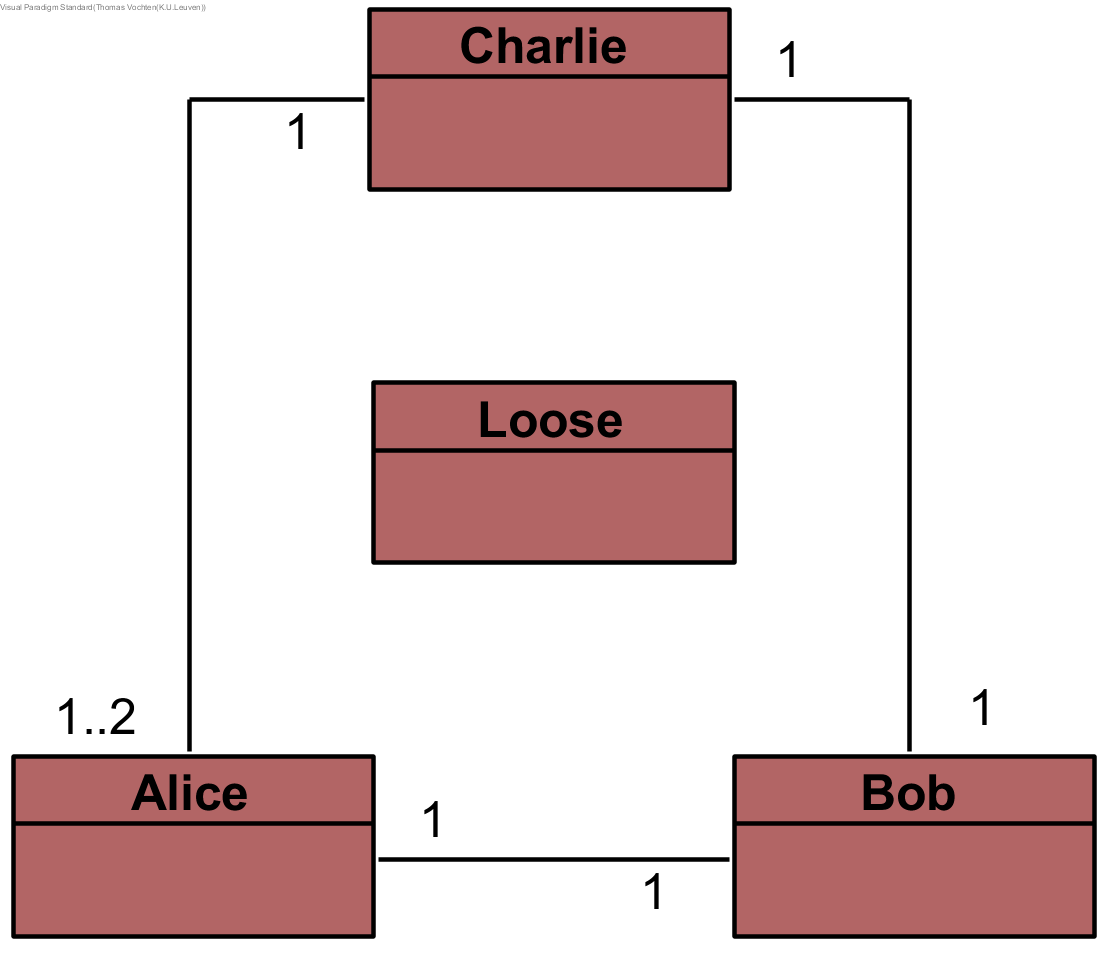
\includegraphics{chap-kwaliteitsgebrek/cycle.png}
	\caption{Voorbeeld van een onvoldoende precieze bovengrens in een klassehi\"erarchie en van een losstaande klasse (zijnde \textit{Loose})}
	\label{fig:cycle}
\end{figure}

\begin{figure}
	\centering
	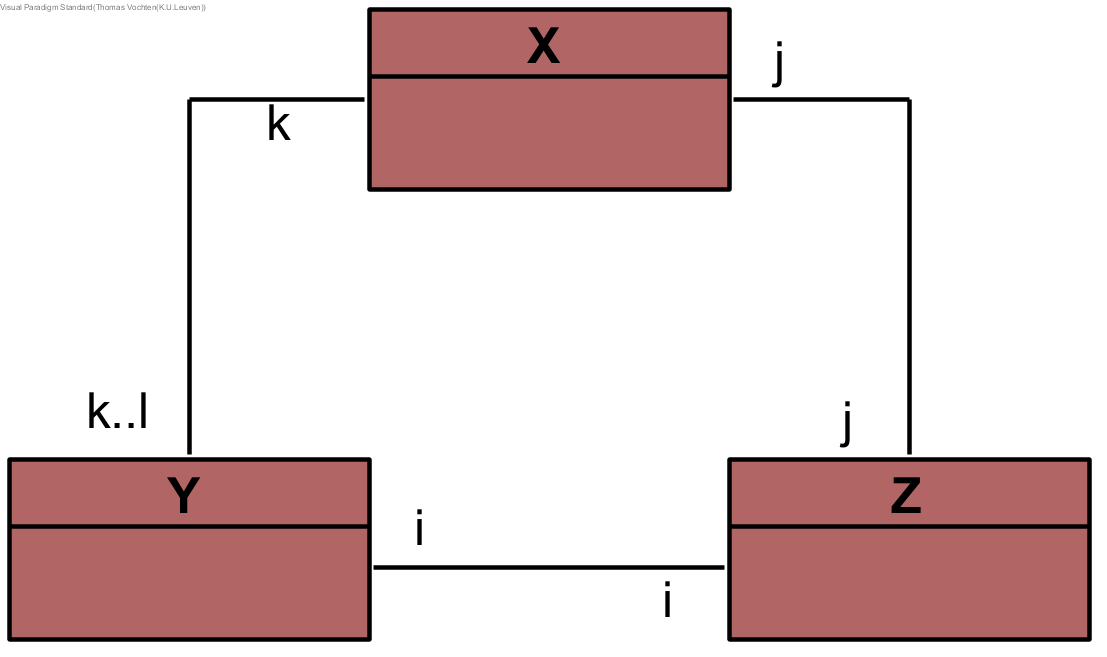
\includegraphics{chap-kwaliteitsgebrek/cyclegen.png}
	\caption{Het algemeen patroon voor onvoldoende precieze bovengrenzen}
	\label{fig:cyclegen}
\end{figure}

Zin \ref{form:manytomany} controleert of voor beide rollen van een associatie geldt dat de bovengrens * is.

Zin \ref{form:loose} controleert of klasse \textit{x} rechtstreeks geassocieerd is met een andere klasse, en zoniet, of klasse \textit{x} een subklasse is van een andere klasse en of die superklasse geassocieerd is met nog een andere klasse.

Zin \ref{form:imprecise-bound} controleert op patronen van associaties zoals in diagram \ref{fig:cyclegen}. De bovengrens op het uiteinde \textit{X} in een associatie \textit{X}---\textit{Y} wordt aangeduid als onvoldoende precies als er aan de volgende voorwaardes wordt voldaan:

\begin{itemize}
	\item \textit{X} en \textit{Y} moeten even veel instanties hebben.
	\item De ondergrens op het uiteinde \textit{X} is gelijk aan $k$ en de ondergrens en bovengrens op het uiteinde \textit{Y} zijn ook gelijk aan $k$.
	\item De bovengrens op het uiteinde \textit{X} is gelijk aan $l > k$ of $*$.
\end{itemize}

Bijlage \ref{app:kwaliteitsgebrek} bevat de theorie die werd gegenereerd uit een combinatie van diagrammen \ref{fig:diagram-voorbeeld} en \ref{fig:cycle}. IDP
vindt alle \textit{many-to-many} associaties en besluit dat \textit{Loose} een losstaande klasse is en verder dat de bovengrens op \textit{Alice} in de associatie \textit{Charlie}---\textit{Alice} onvoldoende precies is.